\documentclass[a4paper]{article}
\usepackage[utf8]{inputenc}
\usepackage[italian]{babel}

\usepackage{tabularx}
\usepackage{natbib}
%\usepackage[demo]{graphicx}
\usepackage{graphicx}

%\usepackage[margin=1.0in]{geometry}

\usepackage{hyperref} %per i link
\usepackage{tikz}

\usepackage{subfigure}
\usepackage{subcaption}
\usepackage{caption}
\usepackage{amsmath, amsthm}

\usepackage{mathrsfs}

\usepackage{pgfplots}
\pgfplotsset{compat=1.18}
\usepackage{caption}

\theoremstyle{definition}
\newtheorem{rich}{richiamo matematico}[section]


%roba che crea comando per centrare immagine dentro immagine piu grande
%https://tex.stackexchange.com/a/308286
\newlength{\imagew}
\newlength{\imageh}
\newlength{\legendw}
\newlength{\legendh}
\newlength{\legendx}
\newlength{\legendy}
\newcommand{\graphicswithlegend}[6]{
	\setlength{\imagew}{#1}
	\settoheight{\imageh}{\includegraphics[width=\imagew]{#2}}
	
	\setlength{\legendw}{#3\imagew}
	\settoheight{\legendh}{\includegraphics[width=\legendw]{#4}}
	
	\setlength{\legendx}{\imagew}
	\addtolength{\legendx}{-\legendw}
	\addtolength{\legendx}{-#5\imagew}
	
	\setlength{\legendy}{\imageh}
	\addtolength{\legendy}{-\legendh}
	\addtolength{\legendy}{-#6\imageh}
	
	\includegraphics[width=\imagew]{#2}%
	\llap{
		\hspace{-\the\legendx}
		\raisebox{\legendy}{\includegraphics[width=\legendw]{#4}}
		\hspace{\the\legendx}
	}
}


\title{Circuiti 1}
\date{Laboratorio di fisica II}
\author{Diana Broggi, Giulia Cantarini, Paolo Falconelli}


\begin{document}

\maketitle


\tableofcontents
\pagebreak
\section {Introduzione}
In questa esperinza abbiamo studiato i circuiti alimentati a corrente continua per verificare alcune leggi fondamentali che caratterizzano componenti quali resistori (conduttori Ohmici) e diodi(semiconduttori, non Ohmici).\\

\section{Strumentazione}
Per costruire i circuiti necessari abbiamo potuto usufruire di:
\begin{itemize}
    \item un alimentatore, per fornire tensione al circuito.
    \item un multimetro da banco utilizzato come Amperometro per la misura delle correnti (data la sua alta sensibilità ai bassi amperaggi).
    \item un multimetro palmare per la misura della tensione applicata (sensibilità 0.001V per voltaggi compresi tra 0.1V e 10V) e delle resistenze(sensibilità variabile).
    \item una breadboard, munita di piste conduttive e di due boccole per l'alimentazione.
    \item dei cavetti con connettore a banana per collegare gli strumenti al circuito.
    \item dei resistori e una scatola delle resistenze variabili(con resistenza interna di 0.2\(\Omega\) ed errore relativo dell'1\% sul valore segnalato).
    \item un diodo.
\end{itemize}

\section{Parte prima}

Inizialmente abbiamo stimato le resistenze parassita di Voltmetro e Amperometro, dal momento che la risoluzione di ogni ciurcuito deve comprendere l'analisi degli effetti degli strumenti di misura sulla corrente che scorre attraverso di essi.\\
In seguito abbiamo eseguito la verifica della legge di Ohm e la misura caratteristica corrente-tensione di due resistori in parallelo ed in serie.


\subsection{Stima resistenza interna del Voltmetro}
\subsubsection*{Metodo adottato}
Supponiamo che la resistenza del Voltmetro sia dell'ordine dei \(M\Omega\), siccome un'alta resistenza interna è un requisito fondamentale per uno strumento di misura che va posto in parallelo al tratto di interesse; per stimarla abbiamo impostato la configurazione in Figura \ref{fig:voltmetro}, scegliendo valori per R che fossero paragonabili a quello atteso per \(R_{V}\).
\pagebreak

\begin{figure}[!ht]

	\makebox[1 \textwidth][c]{       %centering table
		\resizebox{0.5 \textwidth}{!}{   %resize table
			\includegraphics{prima parte/configurazioneI.png}
		} %close resize
	} %close centering
	\caption{}
	  \label{fig:voltmetro}

\end{figure}

\noindent Abbiamo preferito non utilizzare la breadboard, la componente resistiva è stata rappresentata dalla scatola delle resistenze variabili.


\subsubsection*{Dati raccolti}
Abbiamo variato \(R\) utilizzando valori di qualche $M\Omega$, misurato la corrente nel circuito e la tensione ai capi della resistenza, che abbiamo tenuto costante durante tutto il processo.\\
 
\noindent  Per la tensione stimiamo un errore pari a 0.01V, sebbene la sensibilità strumentale fosse dieci volte più piccola. Abbiamo infatti notato che l'ultima cifra variava significativamente durante una singola misurazione, dunque non riteniamo accurata la scelta di una misura eccessivamente precisa. Per l'intensità invece sono state effettuate 4 misure e poi eseguita una media. L'errore sulle resistenze è dato dall'errore strumentale pari all'1\% della misura selezionata.\\


\begin{table}[!htbp]
\centering
    \captionsetup{labelformat=empty}

     \caption{misure per la determinazione di \(R_{V}\)}
    \begin{tabular}{c|c|cccc|c}
        n misura & Resistenza[$M\Omega$] && Intensità& [$\mu A$] && Voltaggio [V]\\
        \hline
        \hline
        \#1& 1.00 \pm 0.01 & 2.475 & 2.478 & 2.476 & 2.477 & 2.29 \pm 0.01\\
        \#2& 4.00 \pm 0.04 & 0.775 & 0.776 & 0.778 & 0.774 & 2.29 \pm 0.01\\
        \#3& 2.50 \pm 0.03 & 1.104 & 1.107 & 1.106 & 1.105 & 2.29 \pm 0.01\\
        \#4& 3.30 \pm 0.03 & 0.901 & 0.902 & 0.903 & 0.904 & 2.29 \pm 0.01\\
        
        \hline
        \hline
    \end{tabular}
\end{table}

\subsubsection*{Analisi dati}

Abbiamo innanzitutto stimato la media e l'errore sulla media associati alle misure dell'intensità con

\[\bar{I}= \frac{\sum{I_{i}}}{N} \hspace{0.5cm} \sigma_{\bar{I}} = \frac{\sigma_{I}}{\sqrt{N}}\]

\noindent notando che l'incertezza risultava sempre inferiore alla sensibilità dello strumento (pari a 0.001\(\mu A\)), abbiamo eseguito i calcoli successivi pondendo \(\sigma_{\bar{I}} = 0.001 \mu A\).

\noindent Così facendo abbiamo stimato la resistenza equivalente del circuito grazie alla legge di Ohm 
\[R_{eq} = \frac{V}{\bar{I}} \hspace{0.5cm} \sigma_{Req} = \sqrt{ \left( \frac{\sigma_{V}}{\bar{I}} \right)^{2} + \left( \frac{V \cdot \sigma_{I}}{ \bar{I}^{2}} \right ) ^{2} }
\]
\noindent Sfruttando la relazione per le resistenze in parallelo abbiamo ottenuto la resistenza parassita del voltmetro, il tutto per ognuna delle resistenza variate nel corso dell'esperimento.

\[\frac{1}{R_{V}} = \frac{1}{R_{eq}} - \frac{1}{R}\] 

\[\sigma_{R_{V}} = \sqrt{  \left( (\frac{R^{2}}{(R - R_{eq})^{2}} \cdot \sigma_{Req} \right )^{2} + \left(\frac{R_{eq}^{2}}{(R_{eq} - R)^{2}}\sigma_{R} \right )^{2} }\]
 
\noindent Riportiamo in tabella i risultati ottenuti:

\begin{table}[!htbp]
\centering
    \captionsetup{labelformat=empty}
\begin{tabular}{c|c|c|c}
        n misura &I[\(\mu A\)] & \(R_{eq} [V]\) & \(R_{V} [V]\)\\
        \hline
        \hline
        $\#$1&2.4765 $\pm$ 0.0006 & 0.923 $\pm$ 0.004 & 12 $\pm$ 2\\
        \hline
        $\#$2&0.7758 $\pm$ 0.0009 & 2.95 $\pm$ 0.01 & 11.3 $\pm$ 0.4\\
        \hline
        $\#$3&1.1055 $\pm$ 0.0006 & 2.071 $\pm$ 0.009 & 12.1 $\pm$ 0.8\\
        \hline
        $\#$4&0.9025 $\pm$ 0.0006 & 2.54 $\pm$ 0.01 & 11.0 $\pm$ 0.4\\
        \hline
        \hline
      	
\end{tabular}
 \caption{per i calcoli abbiamo utilizzato \(\sigma_{I} = 0.001m \mu A\)}
\end{table}

\noindent Alla luce di questi risultati, ognuno affetto dalla sua incertezza, siamo riusciti a stimare la resistenza del voltmetro tramite una media pesata

\[R_V=\sum_{i}^{4}\frac{R_V_i/\sigma^{2}_{R_V_i}}{1/\sigma^{2}_{R_V_i}} \hspace{0.6cm}  \sigma_{R_V}=\sqrt{\frac{1}{\sum_{i}^{4}1/\sigma^{2}_{R_V_i}}}\]

\[\Rightarrow \bar{R_V} = 11.26 \pm 0.06 M\Omega\] 


\subsection{Stima resistenza interna dell'Amperometro}
\subsubsection*{Metodo adottato}

Per stimare la resistenza parassita del multimetro da banco abbiamo cambiato la configurazione del circuito, collegando in serie la resistenza nota e l'amperometro. Questa volta le resistenze selezionate sono dell'ordine di pochi Ohm, per accordarsi con il valore che ci aspettiamo per \(R_{A}\).\\
Sicché il valore indicato sulla resistenza variabile non è accurato in caso di resistenze dell'ordine degli \(\Omega\), ci siamo assicurati, in questi casi, di stimare la resistenza con il multimetro palmare, la cui sensibilità per i valori d'interesse è di 0.1\(\Omega\).

\begin{figure}[!ht]
    \captionsetup{labelformat=empty}

	\makebox[1 \textwidth][c]{       %centering table
		\resizebox{0.5 \textwidth}{!}{   %resize table
			\includegraphics{prima parte/configurazioneII.png}
		} %close resize
	} %close centering
	\caption{Figura 2}
	\label{fig:amperometro}
\end{figure}
\pagebreak

\subsubsection*{Dati raccolti}
La raccolta dati è stata effettuata in maniera analoga all'esperimento precedente.\\

\begin{table}[!htbp]
\centering
    \captionsetup{labelformat=empty}
        \caption{misure per la determinazione di \(R_{A}\)}

    \begin{tabular}{c|c|cccc|c}
        n misura &Resistenza[$\Omega$] && Intensità& [mA] && Voltaggio [V]\\
        \hline
        \hline
        \#1&10.5 \pm 0.1 & 42.871 & 42.871 & 42.869 & 42.870 & 0.55 \pm 0.01\\
        \#2&23.7 \pm 0.1 & 21.035&21.034&21.036&21.036 & 0.55 \pm 0.01\\
        \#3&37.7 \pm 0.1 & 13.677&13.678&13.677&13.678 & 0.54 \pm 0.01\\
        \#4&3.5 \pm 0.1 & 93.901&93.887&93.924&93.918 & 0.54 \pm 0.01\\ 
        
        \hline
        \hline
    \end{tabular}
\end{table}

\subsubsection*{Analisi dati}

Usando la legge di Ohm, abbiamo calcolato la resistenza equivalente e stimato il suo errore

\[R_{eq} = \frac{V}{\bar{I}} \hspace{0.5cm} \sigma_{Req} = \sqrt{ \left( \frac{\sigma_{V}}{\bar{I}} \right)^{2} + \left( \frac{V \cdot \sigma_{I}}{ \bar{I}^{2}} \right ) ^{2} } \]

\noindent Sfruttando la relazione tra le resistenze collegate in serie, abbiamo potuto ricavare la resistenza parassita dell'amperometro e la rispettiva incertezza.

\[R_{A} = R_{eq} - R\]


\[\sigma_{RA} = \sqrt{\sigma_{Req}^{2} + \sigma_{R}^{2}}\]


\pagebreak

\noindent Di seguito riportiamo i risultati ottenuti per ciascuna delle misure:\\


\begin{table}[!htbp]
\centering
    \captionsetup{labelformat=empty}
    \begin{tabular}{c|c|c|c}
        n misura & I[mA] & \(R_{eq}[\Omega]\) & \(R_{A}[\Omega]\)\\
        \hline
        \hline
        \#1& 42.8702 \pm 0.0005 & 12.7 \pm 0.2 & 2.2 \pm 0.3\\
        \hline
        \#2& 21.0353 \pm 0.0005 & 26.0 \pm 0.5 & 2.3 \pm 0.5\\
        \hline
        \#3& 13.6775 \pm 0.0003 & 39.6 \pm 0.7 & 1.9 \pm 0.7\\
        \hline
        \#4& 93.908 \pm 0.008 & 5.8 \pm 0.1 & 2.3 \pm 0.1\\
        \hline
        \hline
    \end{tabular}

     \caption{per i calcoli abbiamo utilizzato \(\sigma_{I} = 0.001m A\)}	
\end{table}

\noindent La miglior stima di $R_A$ è data dalla media pesata dei valori ottenuti e risulta:

\[R_A=\sum_{i}^{4}\frac{R_A_i/\sigma^{2}_{R_A_i}}{1/\sigma^{2}_{R_A_i}} \hspace{0.6cm}  \sigma_{R_A}=\sqrt{\frac{1}{\sum_{i}^{4}1/\sigma^{2}_{R_A_i}}}\]





\[\Rightarrow \bar{R_A} = 2.25 \pm 0.01 \Omega\] 


\subsection{Verifica della legge di Ohm}
La legge di Ohm è una legge sperimentale che regola l'andamento della corrente-tensione caratteristica dei cosiddetti conduttori Ohmici:
\[V = R \cdot I \]

\subsubsection*{Metodo adottato}

Mantenendo la configurazione adottata in precendenza per stimare $R_{V}$, si veda la Figura \ref{fig:voltmetro}, variando la tensione per 20 volte abbiamo misurato l'intensità di corrente I. Con tale set di dati abbiamo potuto tracciare un grafico ed eseguire l'interpolazione necessaria a verificare l'andamento V(I) supposto.

\begin{figure}[!ht]

	\makebox[1 \textwidth][c]{       %centering table
		\resizebox{0.40 \textwidth}{!}{   %resize table
			\includegraphics{prima parte/legge_ohm.png}
		} %close resize
	} %close centering
    \caption{realizzazione in laboratorio del circuito}
  \label{fig:fotoLeggeOhm}
\end{figure}
\noindent Come rappresentato in figura , il Voltmetro è stato posto in parallelo alla resistenza variabile, ipostata su 50\(k\Omega \ll R_{V}\), e la corrente è stata misurata tramite il collegamento in serie (cavo blu di sinistra) con l'Amperometro.


\subsubsection*{Dati raccolti}

Per ogni valore di $V$ impostato, abbiamo raccolto 4 misure di $I$, di cui abbiamo calcolato valor medio e rispettivo errore. Per $V$ stimiamo invece un errore pari a 0.01V, una scelta già discussa in precedenza.


\begin{table}[!ht]
\centering
    \captionsetup{labelformat=empty}
    \caption{dati raccolti per la verifica della legge di Ohm}
    \begin{tabular}{c|cccc|c}
        Voltaggio[V] & &Intensità&[$\mu A$]& & I media [$\mu A$] \\
        \hline
        \hline
        1.50\(\pm 0.01\)&30.140& 30.139& 30.138& 30.140& 30.1393 \(\pm\) 0.0005\\
        2.01\(\pm 0.01\)&40.408& 40.410& 40.411& 40.409& 40.4095 \(\pm\) 0.0006\\
        2.50\(\pm 0.01\)&50.376& 50.375& 50.373& 50.376& 50.375 \(\pm\) 0.0007\\
        2.98\(\pm 0.01\)&60.073& 60.074& 60.075& 60.071& 60.0732 \(\pm\) 0.0009\\
        3.46\(\pm 0.01\)&69.687& 69.688& 69.689& 69.700& 69.691 \(\pm\) 0.003\\
        3.98\(\pm 0.01\)&80.098& 80.097& 80.096& 80.098& 80.0973 \(\pm\) 0.0005\\
        4.47\(\pm 0.01\)&90.122& 90.123& 90.124& 90.121& 90.1225 \(\pm\) 0.0006\\
        4.95\(\pm 0.01\)&99.796& 99.797& 99.794& 99.793& 99.795 \(\pm\) 0.0009\\
        5.48\(\pm 0.01\)&110.353& 110.354& 110.355& 110.357& 110.355 \(\pm\) 0.0009\\
        5.94\(\pm 0.01\)&119.64& 119.63& 119.63& 119.64&  119.635 \(\pm\) 0.003\\
        6.42\(\pm 0.01\)&129.35& 129.36& 129.35& 129.36& 129.355 \(\pm\) 0.003\\
        6.95\(\pm 0.01\)&139.90& 139.89& 139.90& 139.89& 139.895 \(\pm\) 0.003\\
        7.44\(\pm 0.01\)&149.70& 149.71& 149.70& 149.71& 149.705 \(\pm\) 0.003\\
        7.94\(\pm 0.01\)&159.63& 159.62& 159.63& 159.62& 159.625 \(\pm\) 0.003\\
        8.43\(\pm 0.01\)&169.63& 169.62& 169.62& 169.63& 169.625 \(\pm\) 0.003\\
        8.93\(\pm 0.01\)&179.60& 179.61& 179.60& 179.61& 179.605 \(\pm\) 0.003\\
        9.42\(\pm 0.01\)&189.56& 189.55& 189.56& 189.55& 189.555 \(\pm\) 0.003\\
        9.91\(\pm 0.01\)&199.26& 199.27& 199.26& 199.27& 199.265 \(\pm\) 0.003\\
        10.43\(\pm 0.01\)&209.88& 209.92& 209.90& 209.89& 209.897 \(\pm\) 0.009\\
        11.01\(\pm 0.01\)&219.45& 219.46& 219.45& 219.46& 219.455 \(\pm\) 0.003\\
        \hline
        \hline
    \end{tabular}

     \caption{}	
\end{table}


\subsubsection*{Analisi dati}

Abbiamo costruito un grafico di $V$ in funzione di $I$, eseguendo il fit con l'equazione $y=p_{0}x + p_{1}$.\\
Abbiamo tenuto in considerazione le incertezze sulle y, ma anche un errore pari a 0.001$\mu A$ sulle x e propagato ques'ultimo sulle y con la formula \(\sigma^{2}_{y} = \sigma^{2}_{y} + p^{2}_{0}\sigma^{2}_{x}\) (a seguito di una stima preliminare di \(p_{0}\), eseguita trascurando \(\sigma_{x}\)).\\

\noindent Si noti che non tutte le $\sigma_{\bar{I}}$ calcolate in precedenza corrispondono a 0.001\(\mu A\), ma rappresentano ad ogni modo un errore trascurabile rispetto a quello sulle y, quindi trascuriamo questa differenza.

\pagebreak

\begin{figure}[!ht]

	\makebox[1 \textwidth][c]{       %centering table
		\resizebox{0.8 \textwidth}{!}{   %resize table
			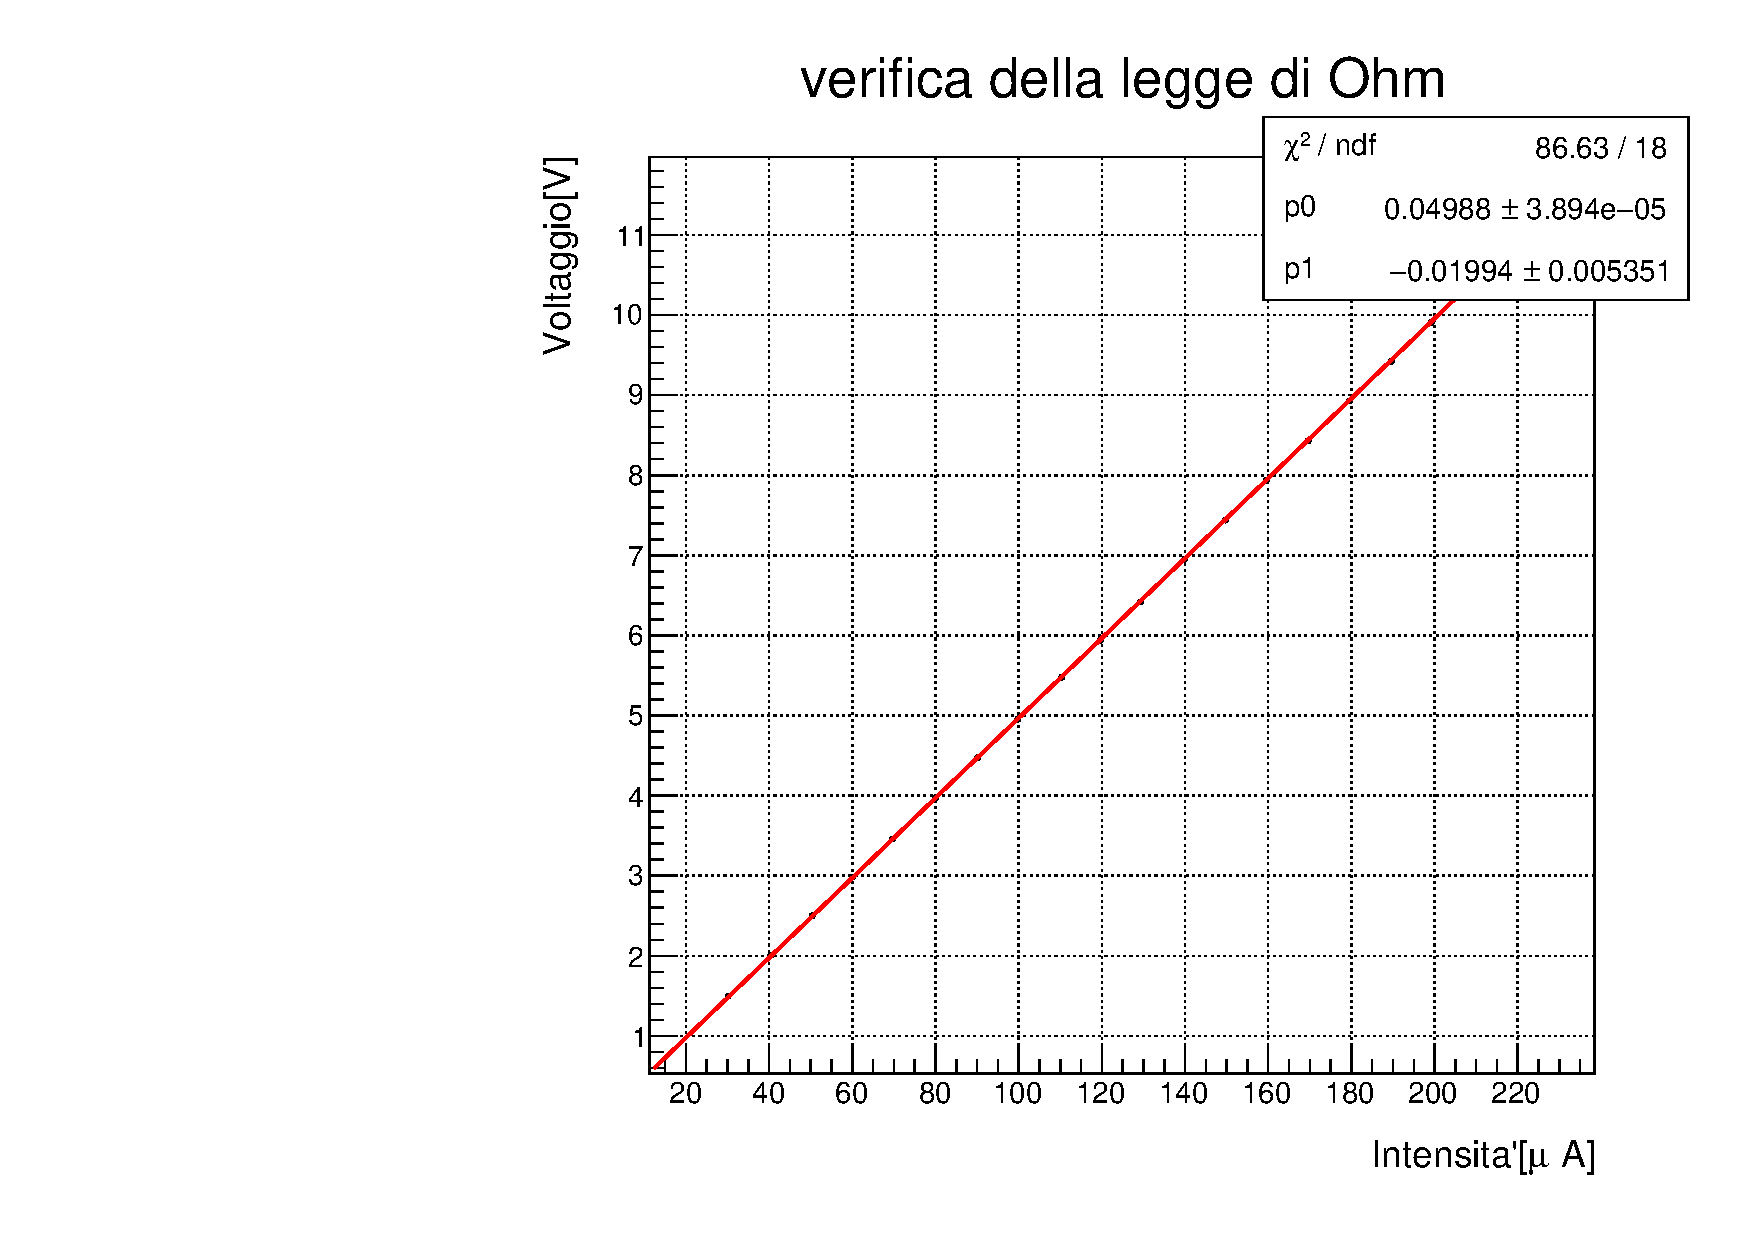
\includegraphics{prima parte/voltaggio_intensita_fit.pdf}
		} %close resize
	} %close centering
	\caption{funzione utilizzata per l'interpolazione: \(y = p_{0}x + p_{1}\)}
	\label{fig:leggeOhm}
\end{figure}

\noindent Il coefficiente angolare della retta risulta \(p_{0} = 49.897 \cdot 10^{-3} \pm 4 \cdot 10^{-6} M\Omega = 49.897 \pm 4 \cdot 10^{-3} k\Omega\); mentre l'intercetta è pari a \(p_{1} = -0.0211 \pm  0.0005 V\),
quindi essendo $\simeq 0$, identifica una retta passante per l'origine, come previsto.\\

\noindent Dal momento che il test del chi quadro non permette di ottenere un risultato accettabile per questo fit, supponiamo di aver sottostimato le incertezze sulle y, possiamo però stimare a posteriori l'errore sulle y grazie alla formula seguente

\[\hat{\sigma_y} = \sigma_y \cdot  \sqrt\frac{\chi^2}{Ndf} \Rightarrow \hat{\sigma_y} = 0.02V\]

\noindent Per concludere questa verifica, osserviamo che il coefficiente angolare stimato corrisponde alla resistenza impostata all'inizio, pari a 50\(k\Omega\), con una probabilità di successo pari all' 11\%:

\[ t = \frac{\left|p_{0} - R\right|}{\sigma_{po}} = \frac{\left |49.897 - 50\right|}{4 \cdot 10^{-3}} = 1.6 \rightarrow PValue = 11\%\]

\noindent Una compatibilità accettabile, ma che sarebbe risultata più soddisfacente se avessimo stimato fin da subito le incertezze sulle y con un valore maggiore. 

\subsection{Misura di resistenze composite}
Al fine di verificare le ben note formule per il calcolo delle resistenze equivalenti di un circuito abbiamo costruito, con l'utilizzo della breadboard, 2 circuiti molto semplici, di cui riportiamo gli schemi in Figura \ref{fig:resParall} e in Figura \ref{fig:resSerie}.

\subsubsection*{Metodo adottato}
Abbiamo scelto 2 resistenze tra quelle a disposizione da poter inserire nella breadboard; la scelta è stata dettata dalla necessità di ottenere una resistenza equivalente notevolmente inferiore rispetto a \(R_{V}\) = resistenza del Voltmetro, precedentemente stimata come \(11.26 \pm 0.06 M\Omega\).\\

\begin{figure}[!h]
\hfill
\subfigure[schema circuito]{\includegraphics[width=7cm]{prima parte/resistenze_in_parallelo.png}}
\hfill
\subfigure[realizzazione in laboratorio]{\includegraphics[width=4cm]{prima parte/res_parall.png}}
\hfill
\caption{resistenze in parallelo}
\label{fig:resParall}
\end{figure}


\begin{figure}[!h]
\hfill
\subfigure[schema circuito]{\includegraphics[width=6cm]{prima parte/resistenze_in_serie.png}}
\hfill
\subfigure[realizzazione in laboratorio]{\includegraphics[width=4cm]{prima parte/res_serie.png}}
\hfill
\caption{resistenze in serie}
\label{fig:resSerie}
\end{figure}

\noindent Abbiamo operato variando il voltaggio del generatore e raccolto i diversi valori di corrente misurati, così da poter ricavare una stima per \(R_{eq}\) da poter confrontare con quella attesa ricavata tramite le formule:


\[ \frac{1}{R_{eq}} = \frac{1}{R_{A}} + \frac{1}{R_{B}} \hspace{0.3cm} (1)  \hspace{2cm}  R_{eq} = R_{A} + R_{B} \hspace{0.3cm}  (2)\]

\subsubsection*{Dati raccolti}

Le resistenze selezionate sono: \(R_{A} = 149.1 \pm 0.1 k\Omega\) e \(R_{B} = 148.7 \pm 0.1 k\Omega\), misurate tramite il multimetro palmare impostato temporaneamente sulla misura di una resistenza.\\

\noindent Riportando il multimetro palmare sull'impostazione per misurare il voltaggio e ruotando la manopola del generatore di tensione, abbiamo ricavato i seguenti valori:

\begin{table}[!htbp]
\centering
    \captionsetup{labelformat=empty}
        \caption{misure per \(R_{A}\) e \(R_{B}\) in parallelo}
    \begin{tabular}{c|cccc|c}
        Voltaggio[V] & & Intensità & [$\mu A$] & & I media[$\mu A$]\\
        \hline
        \hline
        0.94\(\pm 0.01\) & 12.745& 12.747& 12.746& 12.742& 12.745 \(\pm\) 0.001\\
        1.48\(\pm 0.01\) & 19.941& 19.939& 19.940& 19.939 & 19.9397 \(\pm\) 0.0005\\
        2.01\(\pm 0.01\)& 27.201& 27.202& 27.203& 27.200 & 27.2015 \(\pm\) 0.0006\\
        2.50\(\pm 0.01\)& 33.759& 33.757& 33.758& 33.759 & 33.7583 \(\pm\) 0.0005\\
        3.10\(\pm 0.01\)& 41.858& 41.856& 41.854& 41.857 & 41.8563 \(\pm\) 0.0009\\
        3.53\(\pm 0.01\)& 47.768& 47.766& 47.767& 47.768 & 47.7672 \(\pm\) 0.0005\\
        4.18\(\pm 0.01\)& 56.544& 56.545& 56.546& 56.542 & 56.5442 \(\pm\) 0.0009\\
        4.58\(\pm 0.01\)& 61.919& 61.920& 61.918& 61.921 & 61.9195 \(\pm\) 0.0006\\
        5.16\(\pm 0.01\)& 69.768& 69.770& 69.769& 69.771 & 69.7695 \(\pm\) 0.0006\\
        
        \hline
        \hline
    \end{tabular}
    	
\end{table}

\begin{table}[!htbp]
\centering
    \captionsetup{labelformat=empty}
        \caption{misure per \(R_{A}\) e \(R_{B}\) in serie}
    \begin{tabular}{c|cccc|c}
        Voltaggio[V] & & Intensità & [$\mu A$] & & I media[$\mu A$]\\
        \hline
        \hline
        0.72\(\pm 0.01\) & 2.466& 2.467& 2.468& 2.465 & 2.4665\(\pm\)  0.0006 \\
        1.26\(\pm 0.01\) & 4.339& 4.336& 4.337& 4.336 & 4.3370\(\pm\)  0.0007\\
        1.79\(\pm 0.01\) & 6.156& 6.158& 6.159& 6.157 & 6.1575\(\pm\)  0.0006\\
        2.32\(\pm 0.01\) & 7.995& 7.998& 7.994& 7.996 & 7.9958\(\pm\)  0.0009\\
        2.93\(\pm 0.01\) & 10.095& 10.093& 10.092& 10.094 & 10.0935\(\pm\)  0.0006\\
        3.30\(\pm 0.01\) & 11.374& 11.373& 11.375& 11.376 &  11.3745\(\pm\)  0.0006\\
        4.15\(\pm 0.01\) & 14.330& 14.332& 14.329& 14.331 & 14.3305\(\pm\)  0.0006\\
        4.69\(\pm 0.01\) & 16.164& 16.165& 16.163& 16.163 &  16.1638\(\pm\)  0.0005\\
        5.24\(\pm 0.01\) & 18.072& 18.073& 18.071& 18.074 & 18.0725\(\pm\) 0.0006\\
        \hline
        \hline
    \end{tabular}
\end{table}



\subsubsection*{Analisi dati}

Per eseguire i calcoli abbiamo utilizzato \(\sigma_{I} = 0.001\mu A\) pari alla sensibilità dello strumento, dal momento che le fluttauzioni casuali sulle misure non hanno portato ad una stima di errore maggiore.\\
La resistenza equivalente sia per il parallelo che per la serie è stata ottenuta come:

\[\hat{R_{eq}} = \frac{V}{\bar{I}} \hspace{1cm} \sigma_{\hat{R_{eq}}} = \sqrt{ \left ( \frac{\sigma_{V}}{\bar{I}}\right )^{2} + \left( V \frac{ \sigma_{\bar{I}}}{\bar{I}^{2}} \right)^{2} }\]

\noindent e poi confrontata con quella attesa attraverso un test t-Student con limite di accettabilità per PValue fissato a 0.05\%.\\\\\\\\\\\

\noindent La resistenza equivalente attesa per il parallelo è pari a:

\[R_{attesa} = \frac{1}{1/R_A + 1/R_B} = 74.45k\Omega\]
\[ \sigma_{R_{attesa} }= \sqrt{\left(\frac{R^{2}_{B}}{(R^{2}_{B} + R^{2}_{A})^{2}}  \right)^{2}\sigma^{2}_{R_A} + \left(\frac{R^{2}_{A}}{(R^{2}_{B} + R^{2}_{A})^{2}}\right)^{2}\sigma^{2}_{R_B}} = 0.04k\Omega\]


\begin{table}[!htbp]
\centering
    \captionsetup{labelformat=empty}
        \caption{confronto con \(R_{eq} = 74.45 \pm 0.04k\Omega\)}
    \begin{tabular}{c|c|c}
        V/I[k$\Omega$] & t & PVal\\
        \hline
        \hline
        74.0 \(\pm\) 0.8 & 0.6 & 54.9\%\\
        74.0 \(\pm\) 0.5 & 0.9  & 36.8\%\\
        73.9 \(\pm\) 0.4 & 1.4 & 16.2\%\\
        73.9 \(\pm\) 0.3 & 1.8 & 7\%\\
        73.9 \(\pm\) 0.2 &  2.7& 0.7\%\\
        73.9 \(\pm\) 0.2 & 2.7 & 0.7\%\\
        73.9 \(\pm\) 0.2 & 2.7 &0.7\%\\
        73.9 \(\pm\) 0.2 & 2.7 &0.7\%\\
        73.9 \(\pm\) 0.1 & 5 & NA\\
        
        \hline
        \hline
    \end{tabular}
\end{table}

\noindent L'89\% dei test effettuati danno risultato accettabile, quindi possiamo considerare la legge verificata.\\ Notiamo però che all'aumentare del voltaggio, e quindi dell'intensità che attraversa il circuito, la precisione della stima di \(R_{eq}\) aumenta, il che porta a risultati del test sempre meno soddisfacenti. Questo solo perchè la stima di \(R_{attesa}\) non è in realtà accurata: la resistenza equivalente del circuito risulta essere minore per via del parallelo con il voltmetro, che non è stato considerato nella formulazione della legge poichè supposto ininfluente. Considerando infatti il contributo di \(R_{V} = 11.26 M \Omega\): \[\frac{1}{R_{attesa}} = \frac{1}{R_{A}} + \frac{1}{R_{B}} + \frac{1}{R_{V}} \rightarrow R_{attesa} = 73.96 \pm 0.04 k\Omega\]
otteniamo un valore di \(R_{attesa}\) per cui perfino l'ultimo test risulterebbe accettabile con una probabilità del 55\%. In conclusione, la scelta di resistenze inferiori avrebbe ridotto l'influenza del voltmetro e permesso di ottenere una stima accurata con la prima formula, che comunque consideriamo corretta a seguito di questi ragionamenti.

\pagebreak

\noindent La resistenza equivalente attesa per la configurazione in serie è:

\[R_{attesa} = R_{A}+R_{B} = 297.8   k\Omega\]
\[ \sigma_{R_{attesa} } = \sqrt{\sigma^{2}_{RA} + \sigma^{2}_{RB}} = 0.1 k\Omega \]

\noindent tuttavia, dopo quanto osservato precedentemente, ci aspettiamo risultati poco soddisfacenti dall'utilizzo di questa formula. Infatti sommando le resistenze A e B  otteniamo un valore ancora più vicino a quello di \(R_{V}\), dunque quest'ultima sarà ancora più influente nel determinare la stima per \(R_{eq}\) poichè una maggiore percentuale di corrente la attraverserà.\\
Questo disguido sarebbe stato evitabile non solo scegliendo delle resistenze minori come già suggerito ma anche andando a sondare il livello di corrente non in \(I_{1}\) (riferimento a Figura \ref{fig:resSerie}), come eseguito da noi, ma in \(I_{2}\).\\

\noindent Stimiamo dunque nuovamente la resistenza attesa a capo di queste considerazioni, pondendo \(R_{1} = R_{A} + R_{B}\):

\[R_{attesa} = \frac{1}{1/R_{V} + 1/R_{1}} = 290 k\Omega\]
\[\sigma_{R_{attesa}} = \sqrt{\left(\frac{R_V^{2}}{(R_V + R_{1})^{2}}\right)^{2}\sigma^{2}_{R_{1}} + \left(\frac{R_{1}^{2}}{(R_V + R_{1})^{2}}\right)^{2}\sigma^{2}_{R_V}} = 0.1 k\Omega \]

\begin{table}[!htbp]
\centering
    \captionsetup{labelformat=empty}
        \caption{confronto con \(R_{eq} = 290.1 \pm 0.1k\Omega\)}
    \begin{tabular}{c|c|c}
        V/I[k$\Omega$] & t & PVal\\
        \hline
        \hline
        289.9 \(\pm\) 4  & 0.04 & 96.8\%\\
        290.1 \(\pm\) 2 & 0.05 &96\%\\
        289.9 \(\pm\) 2& 0.05 &96\%\\
        289.8 \(\pm\) 1& 0.2 & 84.2\%\\
        289.9 \(\pm\) 1 & 0.1 &92\%\\
        289.9 \(\pm\) 0.9 & 0.1 &92\%\\
        289.9 \(\pm\) 0.7 & 0.1 &92\%\\
        289.9 \(\pm\) 0.6 & 0.2 &84.2\%\\
        289.8 \(\pm\) 0.6 & 0.3 & 76.4\%\\
        
        \hline
        \hline
    \end{tabular}

\end{table}

\noindent Come vediamo, le aspettative sono soddisfatte: le misure rispondono meglio alla seconda formula per \(R_{attesa}\) perciò, sebbene l'esperimento non sia stato eseguito nel modo più convenzionale, abbiamo comunque potuto verificare la corretterzza delle nostre assunzioni sulla composizione di resistori in un circuito CC.

\section{Parte seconda}
Per questa esperinza abbiamo costruito un partitore resistivo e analizzato le sue proprietà variando le resistenze in gioco. \\

\subsection{Partitore resistivo - configurazione senza carico}
Un partitore resistivo è un tipo di circuito costituito da due o più resistenze collegate in serie ai capi delle quali, se viene applicata una tensione, essa si ripartirà sulle stesse in base al loro valore. \\
Nel primo caso sono state utilizzate solo due resistenze, di sotto lo schema del circuito.

\begin{figure}[!ht]

	\makebox[1 \textwidth][c]{       %centering table
		\resizebox{0.70 \textwidth}{!}{   %resize table
			\includegraphics{seconda parte/partitore_resistivo.png}
		} %close resize
	} %close centering
    \caption{}
  \label{fig:partitore}
\end{figure}


\subsubsection*{Metodo adottato}
La scelta dei valori per \(R_{A}\) e \(R_{B}\) è stata determinata da due fattori: la necessità di porre \(R_{B} \ll R_{V}\), al fine di poter misurare la caduta di potenziale su \(R_{B}\) certi che la maggior parte della corrente nel circuito la attraversa; e la richiesta che \(V_{out} \approx 0.5 \cdot V_{in}\), soddisfatta risolvendo il circuito nel seguente modo: \(V_{in} + R_{A}I + R_{B}I = 0\) con \( I = \frac{-V_{out}}{R_{B}}\), allora la condizione da porre è \(V_{in} - R_{A}\frac{V_{in}}{2 \cdot R_{B}} - R_{B}\frac{V_{in}}{2 \cdot R_{B}} = 0 \hspace{0.2cm} \rightarrow \hspace{0.2cm} R_{A = -\frac{1}{2}R_{B}(-2)} \hspace{0.2cm} \rightarrow \hspace{0.2cm} R_{A} = R_{B}\).\\
Abbiamo dunque scelto le resistenze con i valori più simili tra quelle che avevamo a disposizione, costruito il circuito in Figura \ref{fig:partitore} e utilizzato una sonda collegata al multimetro per misurare la caduta di potenziale su \(R_{B}\), prevedendo di ottenere la metà di quella impostata regolando la manopola del generatore. \\

\subsubsection*{Dati raccolti e analisi}
Le resistenze scelte sono: \(R_{A} = 149.1 \pm 0.1 k \Omega\) e \(R_{B} = 148.7 \pm 0.1 k \Omega\), il cui valore è stato valutato tramite il multimetro palmare.\\
\noindent Nella tabella sottostante riportiamo i valori letti per il voltaggio prima e dopo che la tensione venisse ripartita tra le due resistenze.\\
Affianco a ogni dato è riportato il risultato del test t-Student effettuato come segue:
\[t = \frac{\left | V_{in}/2 - V_{out}\right|}{\sqrt{\sigma^{2}_{in} + \sigma^{2}_{out}}}\]
per il PValue associato al test impostiamo un valore minimo per l'accettabilità del 5\%.


\begin{table}[!htbp]
\centering
    \captionsetup{labelformat=empty}
    	 \caption{Res A = 149.1$k\Omega$ ; $\hspace{0.3cm}$ Res B =  148.7$k\Omega$}
    \begin{tabular}{c|c|c|c}

        \(V_{in} [V]\) & \(V_{out} [V]\) & t & PVal \\
        \hline
        \hline
        1.26\(\pm\) 0.01& 0.63\(\pm\) 0.01 & 0.2 & 84.2\%\\
        1.72\(\pm\) 0.01& 0.85\(\pm\) 0.01 & 0.4 & 68.9\%\\
        2.12\(\pm\) 0.01& 1.05\(\pm\) 0.01 & 0.4 & 68.9\%\\
        2.48\(\pm\) 0.01& 1.23\(\pm\) 0.01 & 0.7 & 48.4\%\\
        3.11\(\pm\) 0.01& 1.53\(\pm\) 0.01 & 1.8 & 7.2\%\\
        4.02\(\pm\) 0.01& 1.99\(\pm\) 0.01 & 1.4 & 16.2\%\\
        \hline
        \hline
    \end{tabular}

\end{table}

\noindent Si può osservare che, per le misure raccolte e le incertezze a loro assegnate la previsione era corretta per tutti i casi presi in esame.\\
La diminuizione della compatibilità all'aumentare del voltaggio si può spiegare considerando che la caduta di potenziale non è esattamente la stessa ai capi di \(R_{A}\) e di \(R_{B}\), siccome le due resistenze non hanno lo stesso valore ed \(R_{B}\) è posta in parallelo ad un'altra resistenza. Infatti la caduta di potenziale su \(R_{B}\) è il 49.6\% del potenziale fornito. All'aumentare della corrente complessiva che scorre nel circuito è ragionevole aspettarsi una discrepanza maggiore tra questo 49.6\% ed il 50\%, da cui la diminuizione del PValue osservata.\\
Per una partizione più equa avremmo potuto selezionare \( R_{A}\) ed \(R_{B}\) minori, così da ridurre l'effetto della presenza di \(R_{V}\).
 
\subsection{Partitore resistivo - configurazione con il carico}
Per le misure successive abbiamo aggiunto al nostro partitore delle resistenze di carico, poste in parallelo a \(R_{B}\), per osservare se e come cambiano le proprietà verificate nella prima parte.\\

\subsubsection*{Metodo adottato}
Al fine di verificare che, nell'ipotesi che \(R_{Load} \gg R_{B}\), la caduta di potenziale si spartisce equamente anche con l'aggiunta di resistenze di carico, abbiamo impostato il circuito come mostrato in Figura \ref{fig:partitore2}.\\
Abbiamo inoltre eseguito un confronto con i risultati ottenuti per una \(R_{Load}\) più piccola di \(R_{B}\), per la quale ci aspettiamo che il partitore perda la sua proprietà.

\pagebreak

\begin{figure}[!ht]

	\makebox[1 \textwidth][c]{       %centering table
		\resizebox{0.70 \textwidth}{!}{   %resize table
			\includegraphics{seconda parte/partitore_resistivo2.png}
		} %close resize
	} %close centering
    \caption{}
  \label{fig:partitore2}
\end{figure}

\subsubsection*{Dati raccolti e analisi}
Riportiamo di sotto un confronto tra il caso \(R_{Load} \gg R_{B}\) e \(R_{Load} \ll R_{B}\):\\

\begin{table}[!htbp]
\centering
    \captionsetup{labelformat=empty}
        \caption{Res A = 149.1$k\Omega$ ; $\hspace{0.3cm}$ Res B =  148.7$k\Omega$}
    \begin{tabular}{c|c|c|c|c}
        \(R_{Load}\) & \(V_{in} [V]\) & \(V_{out} [V]\) & t & PVal \\
        \hline
        \hline
        0.893\(\pm\) 0.001 $M\Omega$& 2.77\(\pm\) 0.01 & 1.27\(\pm\) 0.01 & 8 & NA\\
        21.69\(\pm\) 0.01 $k\Omega$& 2.77\(\pm\) 0.01 & 0.31\(\pm\) 0.01  & 78 & NA\\
        
        \hline
        \hline
    \end{tabular}

\end{table}
\noindent Notiamo che il test ha avuto un risultato non accettabile in ognuno dei due casi, questo perchè nel primo caso abbiamo scelto un rapporto \(\frac{R_{Load}}{R_{B}} \approx 10\), evidentemente non sufficiente ad ottenere i risultati sperati. Con un rapporto \(\approx 100\) avremmo soddisfatto le nostre aspettative.\\
Nonostante la pessima scelta di \(R_{A} \)ed \(R_{B}\), che avremmo potuto selezionare tra le resistenze dell'ordine dei \(10\Omega\) per ottenere risultati migliori, da questo esperimento possiamo comunque trarre la conclusione che un partitore è molto più funzionale nel caso \(\frac{\R_{Load}}{R_{B}} \gg 1\) rispetto al caso \(\frac{R_{Load}}{R_{B}} \ll  1 \) che riporta un valore per t 10 volte più grande del precedente.


\subsection{Partitore resistivo - traferimento di potenza sul carico}
Sfruttando il software NI Multisim per la simulazione di circuiti elettronici, abbiamo approfondito la questione relativa al bilancio energetico quando si tratta con circuiti di partizione come quelli descritti fin'ora.\\

\subsubsection*{Metodo adottato}
Per prima cosa abbiamo semplificato il sistema riducendo le resistenze a due sole: \(R_{A}\) e \(R_{Load}\). Assumendo \(V_{g}\) ed \(R_{A}\) fisse, dal momento che stiamo modellizzando un sistema in cui quest'ultima è la resistenza della linea che fornisce corrente, non modificabile e \(V_{g}\) è la tensione applicata dal generatore. Assumendo di poter variariare la resistenza di carico, l'obiettivo è di dimensionare il carico che permette il maggiore trasferimento di potenza su di esso.\\
Abbiamo calcolato \(P_{Load}\), la potenza assorbita dal carico, nel modo seguente: \(P_{Load} = I \cdot V_{Load} = I^{2} \cdot R_{Load}\), stimando \(I = \frac{V_{g}}{R_{a} + R_{Load}}\) siccome le resistenze sono in serie si ottiene:
\[P_{Load} = \frac{V^{2}_{g}}{(R_{Load} + R_{A})^{2}} \cdot R_{Load}\]

\noindent tale funzione presenta un massimo al variare di \(R_{Load}\) in \(R_{Load} = R_{A}\), quindi tale è la resistenza che supponiamo di dover imporre per avere Potenza massima sul carico.\\

\noindent Abbiamo impostato dunque il seguente circuito su Multisim e variato \(R_{Load}\) per accertarci che la potenza calcolata come \(I \cdot V_{RLoad}\) avesse l'andamento atteso.\\


\begin{figure}[!ht]

	\makebox[1 \textwidth][c]{       %centering table
		\resizebox{0.60 \textwidth}{!}{   %resize table
			\includegraphics{seconda parte/partitore_resistivo_approfondimento.png}
		} %close resize
	} %close centering
    \caption{}
  \label{fig:partitore2approfondimento}
\end{figure}

\subsubsection*{Dati raccolti e analisi}

Di seguito i dati rilevati virtualmente:

\begin{table}[!htbp]
\centering
    \captionsetup{labelformat=empty}
        \caption{Res A = 149.1 $k\Omega$}
    \begin{tabular}{c|c|c|c|c}
        \(R_{Load}\) & \(V_{Load}\) & \(I\) & \(P_{Load}\) & \(\%P_{g} \)sul carico \\
        \hline
        \hline
        10$\Omega$ &   26.826 V &  2.682 A & 71.947 W & 0.006\%\\
        50$k\Omega$ &  100.45 kV & 2.009 A & 201.80kW & 25\%\\
        149.1$k\Omega$ & 199.93 kV & 1.342 A & 268.31kW & 50\%\\
        500$k\Omega$ & 308.12 kV & 616.2 mA &  189.88kW & 77\%\\
        1$M\Omega$ &   348.10 kV & 348.1 mA & 121.17kW & 87\%\\
        \hline
        \hline
    \end{tabular}

\end{table}

\noindent Osserviamo che, come atteso, la potenza trasferita sul carico è massima quando \(R_{Load} = R_{A}\). Non è invece vero che tale condizione corrisponde ad un rendimento massimo, poichè all'aumentare della resistenza sul carico la percentuale di potenza del generatore trasferita deve aumentare(rendimento alto per \(\frac{R_{Load}}{R_{A}} \gg 1\)), a costo però di un aumento della resistenza complessiva del circuito, che abbassa il valore netto della potenza sul carico.\\\\

\noindent Nel caso reale, al fine di ridurre il costo complessivo del trasferimento della potenza del generatore \(P_{g}\) al carico, l'obiettivo delle compagnie elettriche è minimizzare la dispersione di potenza per effetto Joule. Siccome l'efficienza, come abbiamo visto, dipende dal rapporto \(\frac{R_{A}}{R_{Load}}\):

\[\frac{P_{Load}}{P_{g}} = \frac{R_{Load}}{(R_{Load} + R_{A})}\]

\noindent per massimizzarla la soluzione che si adotta è porre un trasformatore prima del carico in modo che ricuca \(V_{Load}\) di un fattore \(a > 1\) e aumenti \(I_{Load}\) dello stesso fattore a, così la formula diventa 

\[\frac{P_{Load}}{P_{g}} = \frac{1}{1 + \frac{R_{A}}{R_{Load}a^{2}}}\]
All'aumentare del fattore \(a^{2}\), caratteristico del trasfromatore, la percentuale di \(P_{g}\) trasmessa tende al 100\%.
Per questo motivo vengono utilizzate  alte tensioni per trasportare la corrente, più alto è il fattore di cui devo poi dividere, maggiore sarà l'efficienza della trasmissione.
\pagebreak


\section{Parte terza} %paul
\subsection{Caratterizzazione corrente-tensione di un dispositivo non lineare}
Il diodo è un conduttore la cui caratteristica corrente-tensione non è costante, segue anzi la legge di Shockley:

     \[I = I_{0} \cdot \left(e^{\frac{qV}{gKT}}-1\right) \]

\noindent Lo scopo di questo esperimento è mostrare che la legge di Shockley è soddisfatta e ottenere la cosiddetta \(V_{soglia}\), oltre la quale la corrente condotta dal diodo ha un comportamento lineare rispetto a V.


\subsubsection*{Metodo adottato}
Per l'esecuzione di questo esperimento abbiamo deciso di adottare una configurazione come quella rappresenata nella figura sottostante


\begin{figure}[!ht]

	\makebox[1 \textwidth][c]{       %centering table
		\resizebox{0.50 \textwidth}{!}{   %resize table
			\includegraphics{terza parte/diodo_circuito.png}
		} %close resize
	} %close centering
    \caption{}
  \label{fig:diodo}
\end{figure}

\noindent e raccogliere svariati punti del piano V(I) al fine di poter eseguire un fit del modello sopracitato e di valutare fino a quale \(V_{soglia}\) quest'ultimo si addatta ai dati.

\subsubsection*{Dati raccolti}
L'incertezza che stimiamo per il valore del voltaggio dipende dalla sensibilità del multimetro utilizzato: 0.001V, tuttavia l'errore effettivo potrebbe essere maggiore a causa di fattori che non abbiamo considerato.\\
Invece i valori per l'intensità sono stati rilevati più volte, il che ci porta a stimare le relative incertezze sulle medie come \(\frac{\sigma_{I}}{\sqrt{N}}\).

\pagebreak

 \begin{table}[!htbp]
    	\captionsetup{labelformat=empty}
        \caption{misure effettuate con il diodo }
    \begin{tabular}{c|ccccc}
        tensione [V] &&& intensità [$\mu$A]&& \\
        \hline
        \hline
        0.127\( \pm 0.001\) & 0.012& 0.013& 0.011& 0.013& 0.011\\
        \hline
        0.215\( \pm 0.001\) & 0.030& 0.029& 0.028& 0.028& 0.030\\
        \hline
        0.241\( \pm 0.001\) & 0.040& 0.039& 0.041& 0.039& 0.041\\
        \hline
        0.275\( \pm 0.001\) & 0.073& 0.072& 0.074& 0.072& 0.074\\
        \hline
        0.329\( \pm 0.001\) & 0.263& 0.264& 0.261& 0.262& 0.264\\
        \hline
        0.400\( \pm 0.001\) & 2.043& 2.042& 2.045& 0.049& 2.054\\
        \hline
        0.434\( \pm 0.001\) & 5.966& 5.954& 5.970& 5.951& 5.949\\
        \hline
        0.515\( \pm 0.001\) & 61.090& 61.070& 61.055& 61.056& 61.058\\
        \hline
        0.554\( \pm 0.001\) & 182.12& 182.11& 182.06& 182.07& 182.10\\
        \hline
        0.563\( \pm 0.001\) & 225.59& 225.51& 225.26& 225.30& 225.49\\
        \hline
        0.586\( \pm 0.001\) & 418.86& 418.82& 48.66& 418.76& 418.80\\
        \hline
        0.600\( \pm 0.001\) & 606.55& 606.23& 606.20& 606.45& 606.27\\
        \hline
        0.622\( \pm 0.001\) & 1077.72& 1077.22& 1076.67& 1077.52& 1077.25\\
        \hline
        0.722\( \pm 0.001\) & 12966& 12981& 12988& 12983& 12956\\
        \hline
        0.735\( \pm 0.001\) & 18492& 18491& 18490& 18435& 18408\\
        \hline
        0.744\( \pm 0.001\) & 22943& 22946& 22920& 22906& 22885 \\
        \hline
        0.755\( \pm 0.001\) & 30398& 30418& 30441& 30420& 30383\\
        \hline
        0.765\( \pm 0.001\) & 38805& 38888& 38857& 38863& 38872 \\
        \hline
        0.778\( \pm 0.001\) & 53312& 53331& 53330& 53216& 53210\\
        \hline
        0.782\( \pm 0.001\) & 66722& 66700& 66692& 66681& 66684\\
        \hline
        0.786\( \pm 0.001\) & 79431&  79430& 79466& 79396& 79420\\
        \hline
        0.792\( \pm 0.001\) & 95170& 95320& 95142& 95206& 95171\\
        \hline
        0.800\( \pm 0.001\) & 111119& 111000& 110929& 111154& 111128\\
        \hline
        0.806\( \pm 0.001\) & 152667& 152740& 152848& 152850& 152667\\
        \hline
        0.814\( \pm 0.001\) & 158450& 157510& 156330& 157050& 155300\\
        \hline
        0.825\( \pm 0.001\) & 185900& 187220& 187150& 187540& 187550\\
        \hline
        0.835\( \pm 0.001\) & 235290& 236300& 235870& 236900& 238020\\
        \hline
        0.846\( \pm 0.001\) & 283500& 284400& 284440& 283350& 284160\\
        \hline
        0.856\( \pm 0.001\) & 481220& 481950& 482600& 482330& 486220\\
        \hline
        0.862\( \pm 0.001\) & 620440& 618750& 618350& 620350& 621750\\
        \hline
        0.869\( \pm 0.001\) & 752660& 754120& 755260& 756120& 757280\\
        \hline
        0.879\( \pm 0.001\) & 851240& 851100& 850760& 851230& 852580\\
        \hline
        0.882\( \pm 0.001\) & 973491& 974461& 974463& 989964& 982340\\
        \hline
        0.884\( \pm 0.001\) & 1145290& 1121903& 1162771& 1164579& 1178664\\
        \hline
        0.901\( \pm 0.001\) & 1342800& 1344200& 1346700& 1350200& 1342100\\
        \hline
        0.907\( \pm 0.001\) & 1453022& 1453122& 1442400& 1459300& 1460112\\
        \hline
        0.917\( \pm 0.001\) & 1582034& 1567890& 1542786& 1542768& 1591439\\
        \hline
        0.942\( \pm 0.001\) & 1823300& 1823000& 1818300& 1817300& 1817700\\
        \hline
        0.956\( \pm 0.001\) & 2063900& 2059000& 2058000& 2056000& 2046600\\
        \hline
        0.966\( \pm 0.001\) & 2223460& 2254901& 2243450& 2256790& 2241721\\
        \hline
        \hline
    \end{tabular}

\end{table}

\noindent Alcune misure sono state effettuate in giorni differenti a causa di alcune irregolarità riscontrate nel set di dati, per cui il parametro di temperatura T presente nella legge sopracitata potrebbe aver alterato, seppur in maniera minima la precisione dei dati. 
\subsubsection*{Analisi dati}

Abbiamo deciso di iniziare a raccogliere i dati a partire da una tensione di circa 0.1 V e di arrivare a circa 1 V, con l'accortezza di raccogliere maggiori misure dove ci aspettavamo di incontrare un incremento significativo della curva esponenziale:\\

\begin{figure}[!ht]

	\makebox[1 \textwidth][c]{       %centering table
		\resizebox{0.70 \textwidth}{!}{   %resize table
			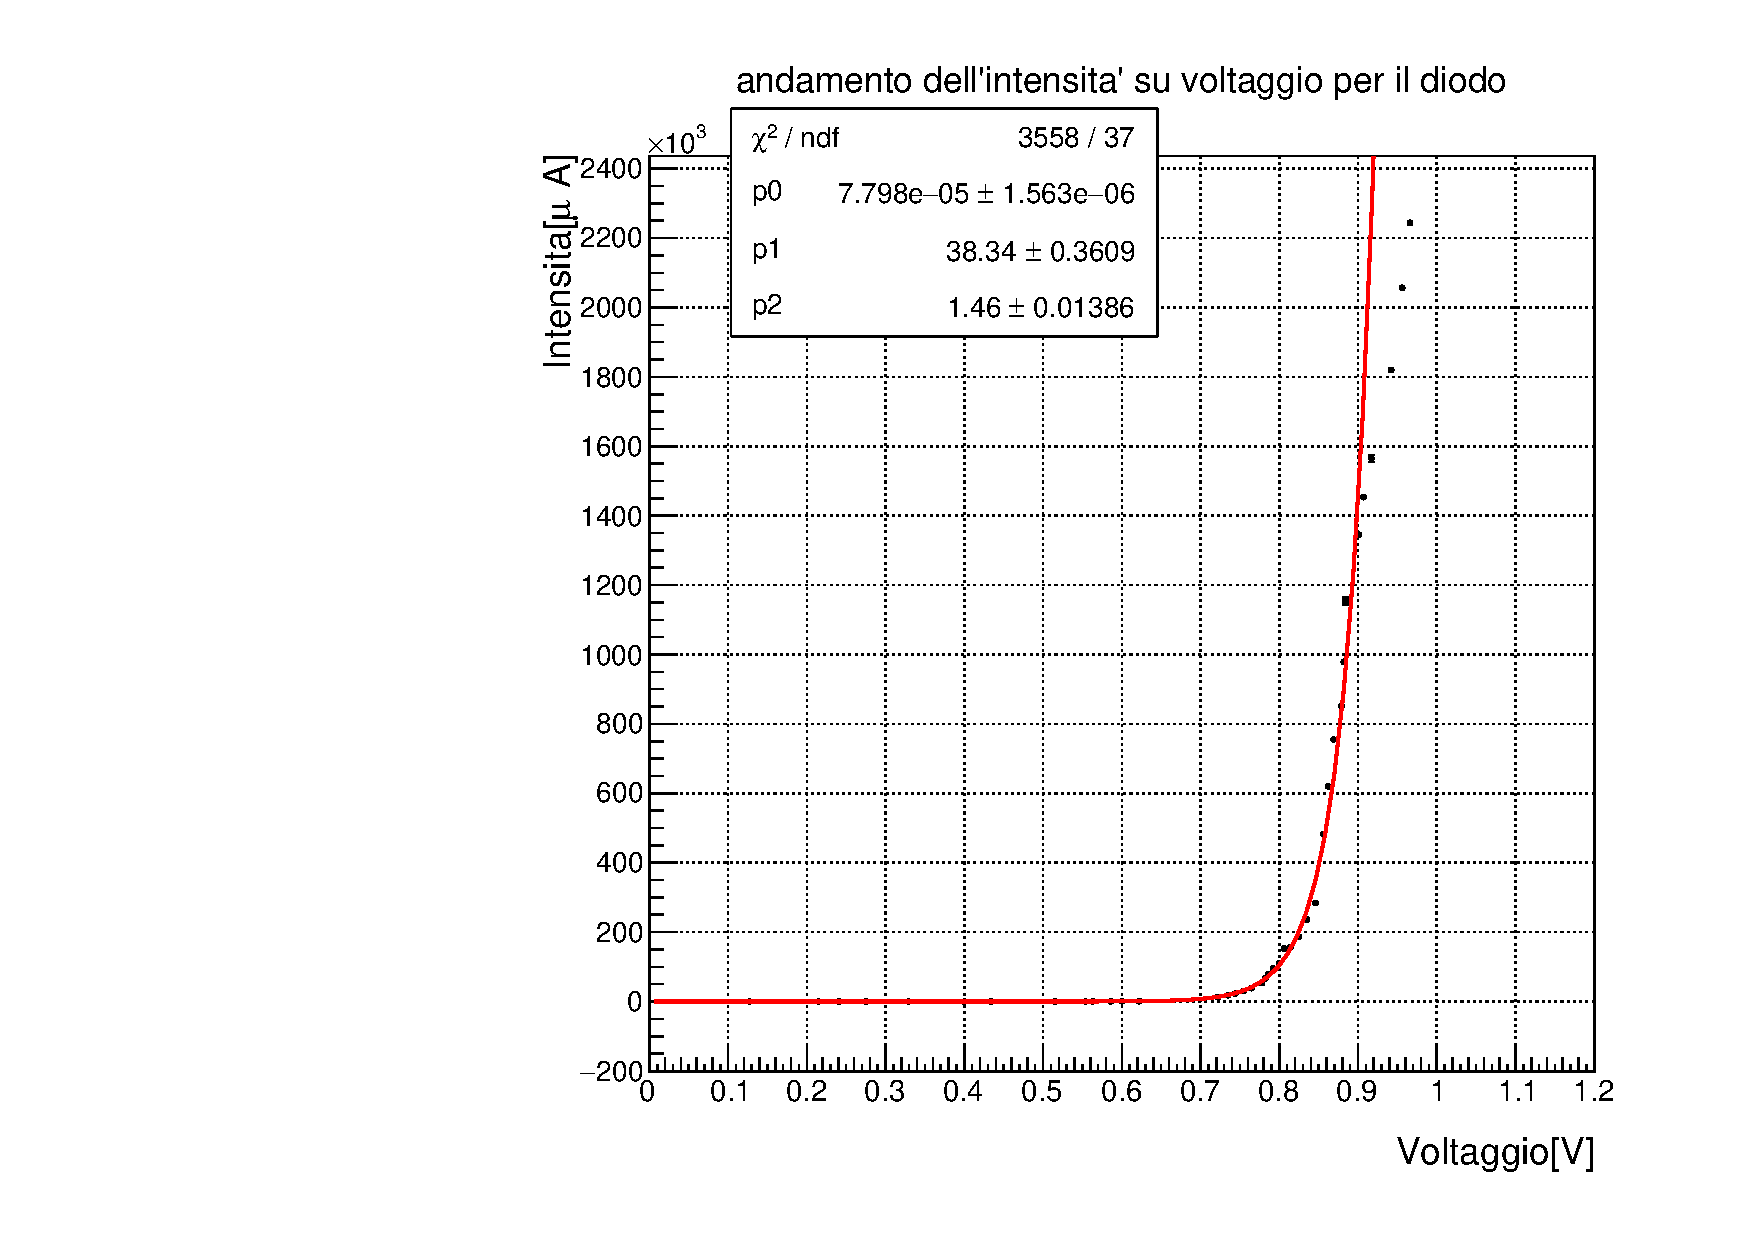
\includegraphics{terza parte/intensita_su_voltaggio.pdf}
		} %close resize
	} %close centering
	\caption{funzione utilizzata per l'interpolazione: \(y = p_{0} e^{\frac{p_{1}x}{p_{2}} }\)}
	\label{fig:intensita_su_voltaggio}

\end{figure}
\noindent come si può ben vedere dal grafico fino a circa 0.9 V si ha una buona approssimazione della legge di Shockley, infatti l'andamento esponenziale è soddisfatto; aumentando il voltaggio invece le misure si distanziano dalla curva per assumere un andamento lineare il che porta ad una stima del \(\chi^{2}\) eccessiva rispetto al numero di gradi di libertà del sistema.\\

\noindent I parametri stimati attraverso il fit sono i seguenti:\\
\( p_{0} = I_{0} = 7.8 \cdot 10^{-5} \pm 2 \cdot 10^{-6} \mu A\),\\
\(p_{1} = \frac{q}{kT} = 38.3 \pm 0.4 V^{-1}\),\\
\( p_{2} = g\) = costante del diodo =  \(1.46 \pm  0.01\).

\pagebreak

\noindent Applicando un'interpolazione lineare ai dati raccolti tra 0.90V e 1.00 V si ottiene una buona approssimazione dell'andamento lineare atteso:\\


\begin{figure}[!ht]
    \captionsetup{labelformat=empty}

	\makebox[1 \textwidth][c]{       %centering table
		\resizebox{0.70 \textwidth}{!}{   %resize table
			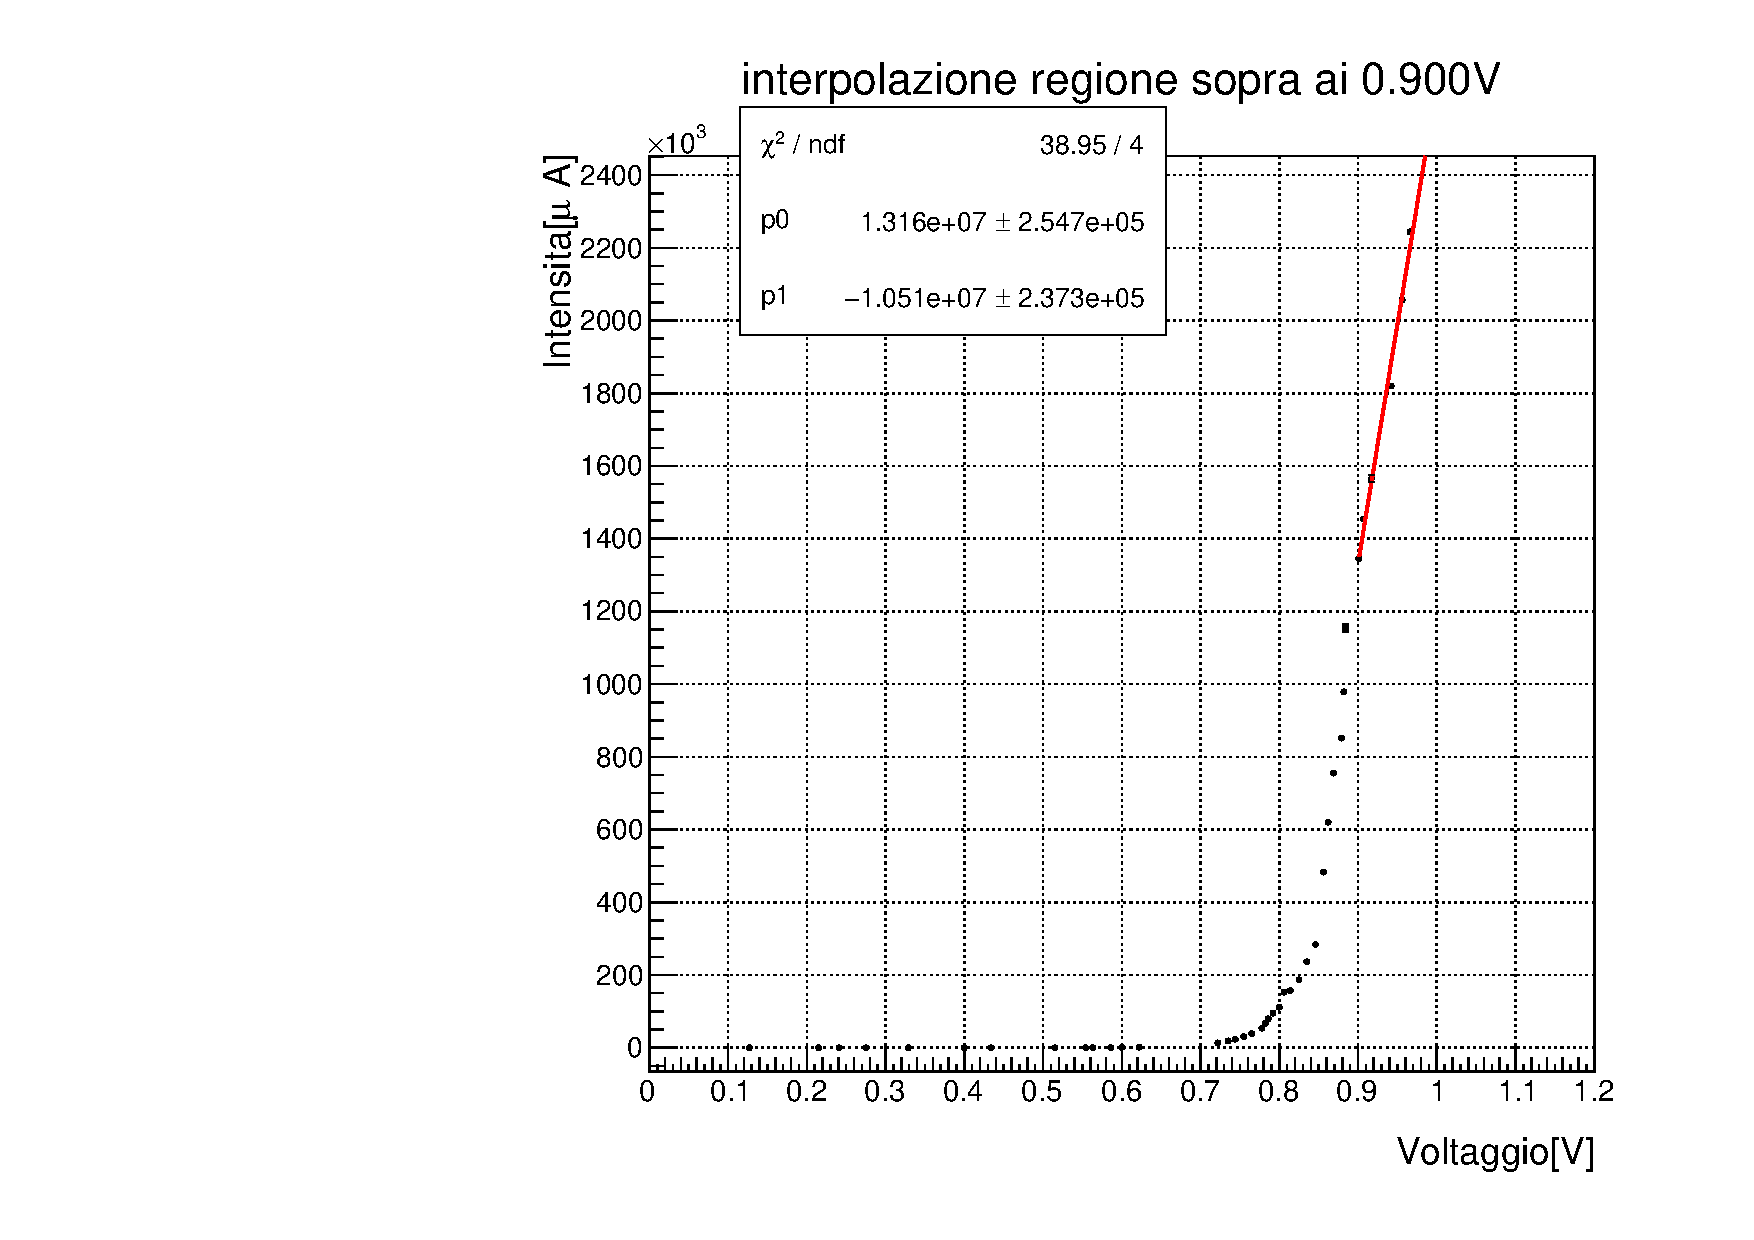
\includegraphics{terza parte/retta_intensita_su_voltaggio.pdf}
		} %close resize
	} %close centering
	\caption{funzione usata per l'interpolazione:\(y = p_{0}x + p_{1}\)}

    \label{fig:retta_intensita_su_voltaggio}

\end{figure}
\noindent Per questa interpolazione parziale il \(\chi ^{2}\) risulta 38.95, da confrontare con il numero dei gradi di libertà ovvero 4. Il PValue per questo risultato non è sufficiente per essere accettabile, attribuiamo questo insuccesso ad una stima degli errori sul voltaggio non veritiera. Infatti siccome il valore riportato come \(\chi^{2}\) corrisponde a:
\[Q^{2}_{0} = \frac{(I - p_{0}V - p_{1})^{2}}{\sigma_{I}^{2} + p_{0}^{2}\sigma_{V}^{2} }\]

il fatto che la stima di \(Q^{2}_{0}\) sia maggiore di 4 ci porta a suppore che il denominatore sia stato valutato in difetto rispetto al valore vero. Notiamo inoltre che il fattore predominante in \(\sigma_{I}^{2} + p_{0}^{2}\sigma_{V}^{2}\) sia quello dato da \(\sigma_{V}\) per via della notevole pendenza \(p_{0}\) della retta. Quindi una stima a posteriori delle incertezze porterebbe a una valutazione più veritiera proprio dell'errore su V.\\
\[\sigma_{V posteriori} = \sqrt{\frac{\chi^{2}}{Ndf}} \sigma_{V} = \sqrt{9.73}\cdot 0.001V = 0.003V\]

\noindent I parametri ottenuti per la retta sono: \\
\(p_{0}\) = coefficiente angolare = \( 1.315 \cdot 10^{7} \pm  3 \cdot 10^{5} \mu \Omega^{-1}\) \\
\(p_{1}\) = intercetta = \( -1.051 \cdot 10^{5}  \pm  2 \cdot 10^{5} \mu A\).\\
Possiamo quindi determinare l'intersezione con l'asse delle ascisse ponendo\\ \(0=p_{0}x1 + p_{1} \rightarrow x1 = \frac{1.051 \cdot  10^{7}}{ 1.315 10^{7}} = 0.7988V \pm   \sigma_{x1}=\sqrt{ \left(\frac{\sigma_{p_{1}}}{p_{0}}\right)^{2} + \left(\frac{\sigma_{p_{0}}p_{1}}{p^{2}_{0}}\right)^{2}}=0.02376V \rightarrow x1 = 0.80 \pm 0.02 V = \hat{V}_{soglia}\).


\end{document}
